%% - Better understanding the theory of attack trees
%% - Specializations using implication
%% - Lina!!
Attack trees are perhaps the most popular graphical model used to
conduct threat analysis of both physical and virtual secure
systems. They were made popular by Bruce Schneier in the late nineties
\cite{Schneier:1999}.  In those early years attack trees were studied
and used as a syntactic tool to help guide analysis.  However, as
systems grew more complex the need for a semantics of attack trees
become apparent; after all, without a proper semantics how can we
safely manipulate attack trees, extend their expressivity, or compare
them?

A number of different models of attack trees have been proposed: a
model in Boolean algebras
\cite{Kordy:2014,Kordy:2012,Pietre-Cambacedes:2010}, series-parallel
pomsets \cite{Mauw:2006}, Petri nets \cite{McDermott:2001}, and tree
automata \cite{Camtepe:2007}.  There have also been various
extensions, such as, adding sequential composition \cite{Jhawar:2015},
and defense nodes \cite{Kordy:2011,Kordy:2012}.  All of these models
and extensions have their benefits, but at the heart of them all is
logic.

The model in boolean algebras was the first and most elegant model of
attack trees, but it failed to capture the process aspect of attack
trees, that is, the fact that base attacks are actual processes that
need to be carried out, and the branching nodes compose these
processes in different ways.  Thus, the community moved towards models
of resources like parallel-series pomsets, Petri nets, and automata.
However, the complexity of these models increased, and hence,
comparing these models becomes difficult. Furthermore, this increased
complexity makes it hard to decide which to use and under which
circumstances.  This difficulty can be resolved by recovering the
elegant logical model of attack trees.

\textbf{Linear Logic.}  It is fitting that attack trees are the most
popular model used in threat analysis, because \emph{linear logic},
one of the most widely studied logics used to reason about resources,
is also an excellent candidate for modeling attack trees.  In fact,
Horne et al.\cite{horne2017semantics} has already produced a number of
interesting results.  Most importantly, they show that attack trees
can be modeled as formulas in linear logic, which then one can prove
properties between attack trees by proving implications between them.
Furthermore, by studying attack trees from a linear logical
perspective they introduce a new property between attack trees called
\emph{specializations}.  Prior to their paper the literature was
primarily concerned with equality between attack trees, but the
logical semantics of attack trees reveal how one can break these
equalities up into directional rewrite rules.  An attack tree is a
\emph{specialization} of another if the former is related to the later
via these rewrite rules.  The logical semantics model the rewrite
rules as implications.

This paper has two main contributions. The first is a new simple
linear logical semantics of causal attack trees -- attack trees with
sequential composition -- in four-valued truth tables.  It comes in
two flavors: the ideal quaternary logic
(Section~\ref{subsec:the_ideal_quaternary_semantics}) and the
filterish quaternary logic
(Section~\ref{subsec:the_filterish_quaternary_semantics}).  These two
types of semantics correspond to truth table semantics for Horne et
al.'s\cite{horne2017semantics} \emph{ideal} and \emph{filter}
semantics of causal attack trees.

\textbf{Functional Programming.} Our second contribution is Lina, a
new domain specific functional programming language for conducting
threat analysis using attack trees.  Consider the example attack trees
in Fig.~\ref{fig:atm-tree}.
\begin{figure}
  \vspace{-10px}
  \begin{tabular}{|l|l|}
    \hline
    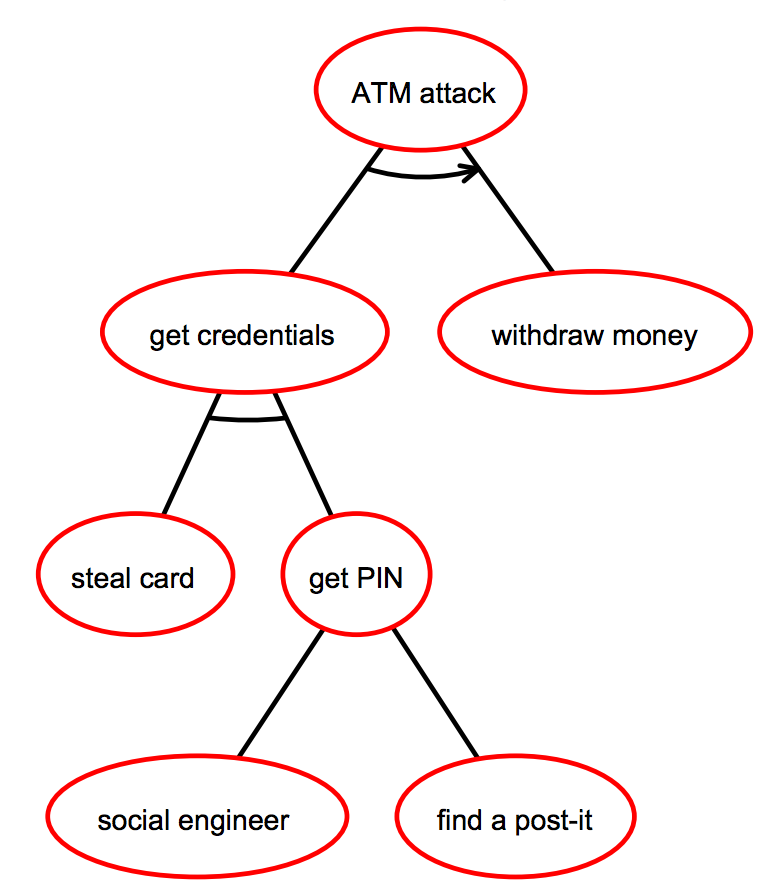
\includegraphics[scale=0.230]{ATM-Tree1}
    &
    \begin{tabular}{l}      
      \begin{minipage}{2.2in}
        \vspace{-200px}
        \begin{minted}[fontsize=\footnotesize]{haskell}
seq_node "ATM attack"
  (and_node "get credentials"
    (base_na "steal card")
    (or_node "get PIN"
      (base_na "social engineer")
      (base_na "find a post-it")))
  (base_na "withdraw money")
        \end{minted}        
      \end{minipage}
    \end{tabular}\\
    \hline
  \end{tabular}
  \\[5px]
  \begin{tabular}{|c|l|}
    \hline
    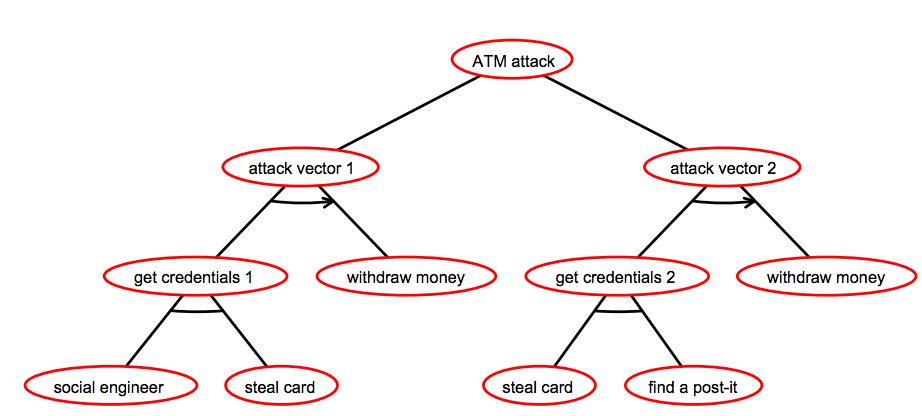
\includegraphics[scale=0.37]{ATM-Tree2}
    \\
    \hline
    \begin{tabular}{l}
      \begin{minipage}{2.5in}
        \vspace{4px}
    \begin{minted}[fontsize=\footnotesize]{haskell}
or_node "ATM attack"
   (seq_node "attack vector 1"
     (and_node "get credentials 1"
       (base_na "social engineer")
       (base_na "steal card"))
     (base_na "withdraw money"))
   (seq_node "attack vector 2"
     (and_node "get credentials 2"
       (base_na "steal card")
       (base_na "find a post-it"))
     (base_na "withdraw money"))
    \end{minted}
    \vspace{4px}
    \end{minipage}
    \end{tabular}\\
    \hline
  \end{tabular}  
  \label{fig:atm-tree}
  \caption{Attack Trees for an ATM attack from Figure~1 and Figure~2 of Kordy et
    al.~\cite{Kordy2017} and their corresponding Lina scripts.}
\vspace{-15px}  
\end{figure}
Both of these contain actual Lina programs for each of the
corresponding attack trees; in fact, every example in this paper is a
Lina program. Lina supports causal attack trees with attributes or
without; thus, there are two types of base attacks: \underline{base}
attacks \underline{w}ith \underline{a}ttributes, denoted
\verb!base_wa!, and \underline{base} attacks \text{w}ith
\underline{n}o \underline{a}ttributes, denoted \verb!base_na!; an
example usage of the former can be found in
Fig.~\ref{fig:vehicle_attack}.  Lina is designed to be extremely
simple, and to reflect the typical pseudocode found throughout the
literature.  However, Lina is more than just a simple definitional
language.

Lina is an embedded domain-specific programming language whose host
language is the Haskell programming language \cite{jones2003haskell}.
So, why Haskell?  As security researchers and professionals, we are in
the business of verifying the correctness of various systems. Thus, we
should be taking advantage of verification tools to insure that our
constructions, tools, and analysis are correct.  By embedding Lina
into Haskell, we are able to take advantage of cutting-edge
verification tools while conducting threat analysis.  For example,
right out the box Lina supports property-based randomized testing
using QuickCheck \cite{Claessen:2011:QLT:1988042.1988046}, and
refinement types in Liquid Haskell
\cite{Vazou:2014:RTH:2692915.2628161} to verify properties of our
attack trees or the attribute domains used while analyzing attack
trees.  Furthermore, Haskell's advanced type system helps catch bugs
while we develop our attack trees and their attribute domains as a
side-effect of type checking.  Finally, functional programs are short,
but not obfuscated, and hence allow for very compact and trustworthy
programs.

That being said, we are designing Lina so that it can be used with
very little Haskell experience.  It is our hope that one will be able
to make use of Lina without knowing Haskell, and we plan to develop
new tooling to support this.

Lina approaches threat analysis from a programming language
perspective, leading to a number of new advances.  First, as
Gadyatskaya and Trujillo-Rasua \cite{10.1007/978-3-319-74860-3_9}
argue, as a community we need to start building more automated means
of conducting threat analysis, and there is no better way to build or
connect automated tools than a programming language.  Lina is perfect
as a target for new tools, and it can be connected to existing tools
fairly easily.  In fact, Lina already supports automation using the
automatic rewrite system Maude \cite{clavel2005maude}; for example,
the two attack trees in Fig.~\ref{fig:atm-tree} can be automatically
proven equivalent to each other in Lina.  This is similar to Kordy's
\cite{Kordy2017} SPTool, but Lina goes further and supports more than
one backend rewrite system; for example, Lina is the first tool to
support automatically proving specializations of attack trees.  The
user can choose which backend they wish to use.

%%% Local Variables: 
%%% mode: latex
%%% TeX-master: main.tex
%%% End: 
